\documentclass[sigconf,anonymous,review]{acmart}

% Submission settings. The ACM reference block and rights notice are switched off to keep the 4-page body;
% restore them for the camera-ready version.
\settopmatter{printacmref=false}
\setcopyright{none}
\renewcommand\footnotetextcopyrightpermission[1]{}
\acmConference[WSDM '27]{The 20th ACM International Conference on Web Search and Data Mining}{February 15--19, 2027}{Hong Kong}

\usepackage{booktabs}
\usepackage{xspace}

\newcommand{\Qhat}{\ensuremath{\hat Q}\xspace}
\newcommand{\muz}{\ensuremath{\hat\mu_0}\xspace}
\newcommand{\TY}{T+Y\xspace}
\newcommand{\pp}{\,pp\xspace}
\newcommand{\ci}[2]{\,[#1,\,#2]}

\begin{document}

\title{Outcome Composition Can Invert Do-PFN's Uplift Ranking:\\A Criteo Case Study}

\author{Anonymous Author(s)}
\affiliation{\institution{Anonymous Institution}\country{}}

\begin{abstract}
Causal foundation models such as Do-PFN and CausalPFN estimate treatment effects in context: they read a sample of labelled rows and score new users without training. For uplift targeting on large logs, the rows that fill the context are a design choice that papers rarely report. On the Criteo uplift benchmark, whose visit outcome occurs for about 4\% of users, the released Do-PFN checkpoint ranks users in the wrong direction when its 1,024-row context follows the natural outcome rate: normalized Qini is $-0.077$ in cross-validation and $-0.046$ on a 2.09M-row holdout. Balancing outcomes within each treatment arm reverses the sign without retraining ($+0.056$ and $+0.048$). The inversion lies in how Do-PFN reads the context, not in the rows: CausalPFN, a TabPFN T-learner and classical learners fitted on the same rows do not invert. Across outcome shares, the sign of Do-PFN's ranking tracks how its scores align with baseline visit risk, where Criteo's uplift is concentrated. A 20\% share tuned on cross-validation beats balancing on the holdout in all 10 contexts tried ($+0.025$ in normalized Qini), but it does not transfer to a second dataset.
\end{abstract}

\begin{CCSXML}
<ccs2012>
<concept><concept_id>10010147.10010178.10010187.10010192</concept_id>
<concept_desc>Computing methodologies~Causal reasoning and diagnostics</concept_desc><concept_significance>500</concept_significance></concept>
<concept><concept_id>10002951.10003260.10003272</concept_id>
<concept_desc>Information systems~Online advertising</concept_desc><concept_significance>300</concept_significance></concept>
</ccs2012>
\end{CCSXML}
\ccsdesc[500]{Computing methodologies~Causal reasoning and diagnostics}
\ccsdesc[300]{Information systems~Online advertising}

\keywords{uplift modeling, causal foundation models, in-context learning, prior-data fitted networks, class imbalance}

\maketitle

\section{Introduction}

\begin{figure*}[t]
  \centering
  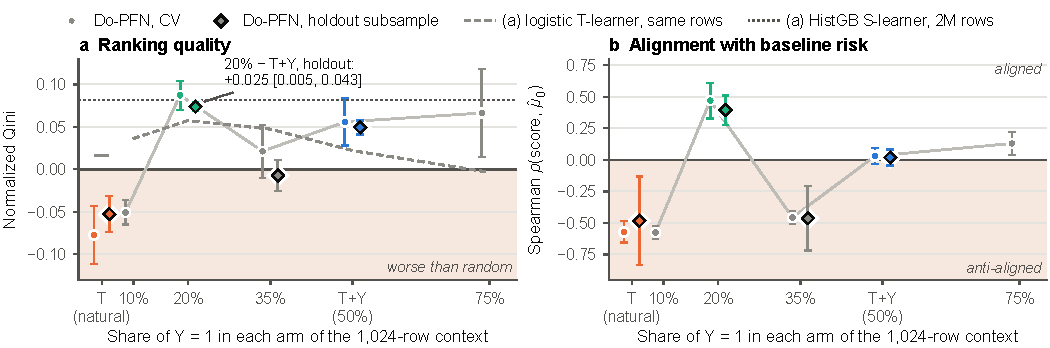
\includegraphics[width=\textwidth]{figures/fig1_share.pdf}
  \caption{Do-PFN against the share of visitors ($Y{=}1$) in each treatment arm of a 1,024-row Criteo context. Circles show CV fold means with 95\% fold-level $t$-intervals; diamonds show the 200k-row holdout subsample with $t$-intervals over contexts (3 contexts for T and 35\%, 10 for 20\% and \TY). (a)~Ranking quality. The shaded region marks rankings worse than random. The dashed line shows a logistic T-learner fitted on the same context rows; the dotted line shows a HistGB S-learner fitted on 2M development rows. (b)~Rank correlation of Do-PFN's scores with estimated baseline risk \muz. Do-PFN inverts exactly where its scores are anti-aligned with risk, except at 35\% in CV.}
  \label{fig:share}
\end{figure*}

Uplift models rank users by how much a treatment, such as an ad impression or a coupon, changes their chance of acting, so that a campaign reaches the users it persuades~\cite{gutierrez2017review,devriendt2018survey}. The usual practice is to fit a meta-learner for each campaign~\cite{kunzel2019metalearners}. Causal prior-data fitted networks (PFNs) offer another workflow. Do-PFN~\cite{robertson2025dopfn} and CausalPFN~\cite{balazadeh2025causalpfn} are pretrained on simulated causal data. Like the TabPFN classifiers they build on~\cite{hollmann2023tabpfn,hollmann2025accurate}, they read a context of labelled rows $(x,t,y)$ and return effect estimates for new users in one forward pass. On web-scale logs the context is a tiny sample: here 1,024 of almost 12 million development rows. The sampler that fills it is therefore part of the method.

For rare binary outcomes the sampler matters. Case-control sampling, which over-represents positives, shifts the intercept of a logistic model but leaves its slopes intact~\cite{prentice1979casecontrol,king2001rare,fithian2014local}. In uplift modeling, undersampling the majority class helps some learners and hurts others~\cite{nyberg2021imbalance,nyberg2023exploring}. For PFN classifiers, downsampling the majority class works about as well as the best correction~\cite{mcdowell2026imbalance}. We ask the same question for causal PFNs and get a sharper answer than ``balancing helps''.

On the Criteo uplift benchmark~\cite{diemert2021criteo}, about 4\% of users visit. When the context follows this natural rate, the released Do-PFN checkpoint ranks users backwards: its normalized Qini is negative in every cross-validation fold and on a frozen 2.09M-row holdout. We fill each treatment arm of a context of the same size with equal numbers of visitors and non-visitors (within-arm outcome balancing). This turns the sign positive without retraining (Fig.~\ref{fig:share}a). Four research questions organize the evidence:
\begin{itemize}
\item[\textbf{RQ1}] Does the outcome composition of a fixed-size context, rather than its size, set the sign of Do-PFN's uplift ranking? Does the repair hold on a holdout?
\item[\textbf{RQ2}] Is the inversion a property of the context rows or of the model that reads them?
\item[\textbf{RQ3}] Does the sign track how Do-PFN's scores align with baseline risk?
\item[\textbf{RQ4}] Can the outcome share be tuned into a reliable, competitive ranker?
\end{itemize}

We contribute a diagnosis and a cheap repair for a public causal foundation model. First, on Criteo the outcome share of the context sets the sign of Do-PFN's ranking at every context size we tried, and balancing reverses it on a frozen holdout ($\Qhat$ $-0.046 \to +0.048$). Second, the inversion lies in how Do-PFN reads the context: two other PFNs and two classical learners fitted on the same 1,024 rows do not invert. Third, the inversion coincides with scores anti-aligned with baseline risk, while Criteo's uplift sits among the highest-risk users. Fourth, a share tuned on cross-validation improves on balancing out of sample but does not transfer to another dataset. The sampler itself is standard. What is new is that its choice flips the sign of a causal PFN's ranking. Do-PFN documents continuous outcomes as its regime, so our results describe the released checkpoint on a standard binary benchmark; they do not refute the method.

\section{Setup}

\textbf{Data.} Criteo uplift v2.1~\cite{diemert2021criteo} pools randomized ad-exposure trials: 13.98M users, about 85\% treated, anonymized features and a binary visit outcome. The cleaned copy used in this project lacks two of the 12 features (f7, f10). A random 15\% holdout (2,093,918 rows) was set aside before modeling. On it, treated users visit at 4.87\% and controls at 3.86\%, an average effect of $+1.01$\pp. The other rows form five cross-validation (CV) folds, grouped so that identical feature vectors never cross folds; each fold is evaluated on 8,000 of its rows. As a second dataset we use LZD, the Lazada data released with DESCN~\cite{zhong2022descn}.

\textbf{Models.} \emph{Do-PFN}~\cite{robertson2025dopfn}, released checkpoint. The binary outcome is its regression target (z-scored, as the official interface does), and a user's score is $\hat\tau(x)=\hat{\mathrm{E}}[Y\mid do(T{=}1),x]-\hat{\mathrm{E}}[Y\mid do(T{=}0),x]$. \emph{CausalPFN}~\cite{balazadeh2025causalpfn}, released checkpoint. A \emph{TabPFN T-learner}~\cite{hollmann2025accurate}, one TabPFN classifier per arm. As controls fitted on exactly the same context rows, a \emph{logistic T-learner} and a histogram gradient-boosting (\emph{HistGB}) \emph{S-learner}.

\textbf{Context designs.} Each context holds $K$ rows from the training fold; for the holdout they come from development rows. \emph{R} samples uniformly. \emph{T} takes half treated and half control rows, with outcomes at their natural rate of about 4\%. \emph{\TY} makes half the rows in each arm visitors. \emph{Share $s$} makes a fraction $s$ of each arm visitors, so \TY is $s{=}50\%$. Any design with equal shares in both arms sets the context's average effect to exactly zero. A useful ranking must then come from heterogeneity, not from the average. We use $K{=}1{,}024$ and check $K$ from 512 to 4,096. Larger contexts, as used for CausalPFN, were beyond our GPU budget.

\textbf{Metrics.} We report normalized Qini \Qhat~\cite{radcliffe2007qini}, AUUC and uplift@10\%: the treated minus control visit rate among the 10\% top-scored users, in percentage points (pp). In CV we average three context seeds per fold and report a $t$-interval over the five folds. On the holdout we report a $t$-interval over context seeds. A cluster bootstrap over identical feature vectors gives a secondary, row-level interval~\cite{bokelmann2024improving}. To relate scores to baseline risk, we fit HistGB per arm on 2M development rows disjoint from all evaluated rows, which gives $\muz(x)$. We then report the Spearman correlation $\rho(\hat\tau,\muz)$.

\textbf{Holdout use.} The comparison of T and \TY on the full holdout was run once. To save compute, the share follow-up (RQ3--4) uses a fixed random subsample of 200k holdout rows. Its hypotheses were written into an internal protocol shortly before the runs, without a hash. The holdout had served other comparisons earlier in the project. We therefore treat it as held out from tuning, not as untouched.

\section{RQ1: Composition sets the sign}

\begin{figure*}[t]
  \centering
  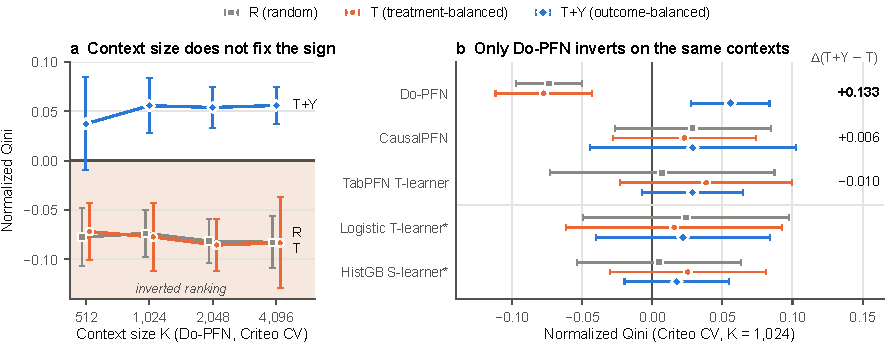
\includegraphics[width=\textwidth]{figures/fig2_models.pdf}
  \caption{Criteo CV, 5 folds, 95\% fold-level $t$-intervals. (a)~Do-PFN's normalized Qini against context size: R and T contexts invert at every $K$; outcome-balanced (\TY) contexts do not. (b)~The same $K{=}1{,}024$ contexts read by three foundation models and by two learners fitted on those rows (*). Only Do-PFN inverts, and only Do-PFN gains from outcome balancing; the right column gives that gain.}
  \label{fig:models}
\end{figure*}

Under R or T contexts, Do-PFN's normalized Qini is negative at every context size: $-0.072$ to $-0.085$ for $K$ from 512 to 4,096. Under T at $K{=}1{,}024$ it is $-0.077$, negative in all five folds and in 14 of 15 runs. Quadrupling the context does not help, so the context's size is not the problem (Fig.~\ref{fig:models}a). Outcome balancing gives $+0.037$ to $+0.056$ at the same sizes. At $K{=}1{,}024$ the gain over T is $+0.133$\ci{0.102}{0.165} (Fig.~\ref{fig:models}b).

The repair holds out of sample (Table~\ref{tab:holdout}). On all 2.09M holdout rows, \Qhat rises from $-0.046$ under T to $+0.048$ under \TY. The gain is $+0.094$\ci{0.037}{0.150} over three contexts per design, and AUUC gains $+0.037$\ci{0.015}{0.059}. The gain of 1.8\pp in uplift@10\% is not resolved with three contexts ($[-1.3,\,4.9]$). The raw predictions show the size of the error. Under T, 94--97\% of Do-PFN's effect predictions on the holdout are negative (medians $-0.17$ to $-0.40$\pp), although treatment raises visits by 1.01\pp on average. Under \TY about a quarter are negative.

\begin{table}[t]
  \caption{Do-PFN on the frozen Criteo holdout, $K{=}1{,}024$. Rows show means over $n$ contexts; contrasts show 95\% $t$-intervals over contexts. Reference learners are fitted on 2M development rows.}
  \label{tab:holdout}
  \small
  \setlength{\tabcolsep}{4pt}
  \begin{tabular}{@{}lrrrr@{}}
    \toprule
    Design & $n$ & \Qhat & AUUC & up@10\% (pp) \\
    \midrule
    \multicolumn{5}{@{}l}{\emph{Full holdout, 2,093,918 rows}} \\
    T & 3 & $-0.046$ & $-0.018$ & 1.76 \\
    \TY & 3 & $0.048$ & $0.019$ & 3.56 \\
    \TY $-$ T & & \textbf{+0.094} & +0.037 & +1.80 \\
    & & \footnotesize{[0.037, 0.150]} & \footnotesize{[0.015, 0.059]} & \footnotesize{[$-$1.3, 4.9]} \\
    \midrule
    \multicolumn{5}{@{}l}{\emph{Fixed 200k-row subsample}} \\
    T & 3 & $-0.053$ & $-0.021$ & 1.43 \\
    35\% & 3 & $-0.007$ & $-0.003$ & 2.12 \\
    \TY & 10 & $0.049$ & $0.019$ & 3.50 \\
    20\% & 10 & $0.074$ & $0.029$ & 4.67 \\
    20\% $-$ \TY & & \textbf{+0.025} & +0.010 & +1.17 \\
    & & \footnotesize{[0.015, 0.034]} & \footnotesize{[0.006, 0.014]} & \footnotesize{[0.32, 2.02]} \\
    35\% $-$ 20\%\,($n{=}3$) & & $-0.082$ & $-0.033$ & $-3.11$ \\
    & & \footnotesize{[$-$0.107, $-$0.058]} & \footnotesize{[$-$0.042, $-$0.023]} & \footnotesize{[$-$4.3, $-$1.9]} \\
    \midrule
    HistGB S-learner & -- & $0.082$ & $0.032$ & 5.36 \\
    HistGB T-learner & -- & $0.079$ & $0.031$ & 5.28 \\
    \bottomrule
  \end{tabular}
\end{table}

\section{RQ2: The model, not the rows}

If T contexts simply lacked information about who responds, every learner that reads them should fail. They do not (Fig.~\ref{fig:models}b). On the same contexts, CausalPFN and the TabPFN T-learner do not rank backwards under R or T, and balancing changes their \Qhat by only $+0.006$ and $-0.010$. Do-PFN's gain from balancing exceeds theirs by $+0.127$\ci{0.044}{0.210} and $+0.143$\ci{0.062}{0.223} (fold-level interaction). The two classical learners fitted on exactly the same 1,024 rows also stay at or above zero ($+0.005$ to $+0.025$). Under R and T they beat Do-PFN in 12--14 of 15 paired runs. The rows therefore carry a usable, if weak, signal, and the inversion arises in how Do-PFN reads them. The control intervals are wide (8,000 evaluation rows per fold), so Fig.~\ref{fig:models}b shows that no other model inverts; it does not rank the controls. The TabPFN T-learner gains nothing from balancing, which also separates our finding from downsampling for PFN classifiers~\cite{mcdowell2026imbalance}. Here, balancing does not improve PFNs in general.

\section{RQ3: Three alignment states}

Fig.~\ref{fig:share} varies the visitor share of each arm with $K$ fixed. Do-PFN's response is not monotone. In CV, \Qhat is $-0.051$ at 10\%, peaks at $+0.087$ at 20\%, dips to $+0.021$ at 35\%, and recovers to $+0.056$ and $+0.066$ at 50\% and 75\%. The dip is reproduced on the holdout: 35\% scores $0.082$\ci{0.058}{0.107} below 20\%, in every context. The logistic T-learner on the same rows stays between 0 and 0.06 at every share.

The sign tracks one property of the scores: their rank correlation with estimated baseline risk \muz (Fig.~\ref{fig:share}b). The designs fall into three states. \emph{Anti-aligned} (R, T, 10\%, 35\%): $\rho<0$ in all 15 CV runs of each design and in every holdout context for T and 35\% ($\rho\approx-0.47$). \emph{Aligned} (20\%): $\rho>0$ in all 15 CV runs and in all 10 holdout contexts (mean $+0.39$). \emph{Neutral} (\TY): $\rho\approx0$ ($+0.03$ in CV, $+0.02$ on the holdout).

Fig.~\ref{fig:anatomy} shows why this alignment decides the sign on Criteo. The observed uplift is concentrated among high-risk users: 2.4 and 4.3\pp in the top two deciles of \muz, and close to zero below decile 8. Under T, Do-PFN places the top decile at a mean score percentile of 24, among the users it would target last. \TY moves this decile to 63, and the 20\% design to 87. Where uplift grows with risk, anti-aligned scores invert the ranking. Neutral scores rank by the remaining heterogeneity, and aligned scores add the risk gradient.

We present this as an association, not a mechanism. Two cases break a simple rule: at 35\% in CV, $\rho$ is negative while \Qhat is positive, and on LZD $\rho$ and \Qhat are unrelated. Explaining why Do-PFN's scores change their relation to risk as the share moves would need separate per-arm predictions, which we leave open.

\begin{figure}[t]
  \centering
  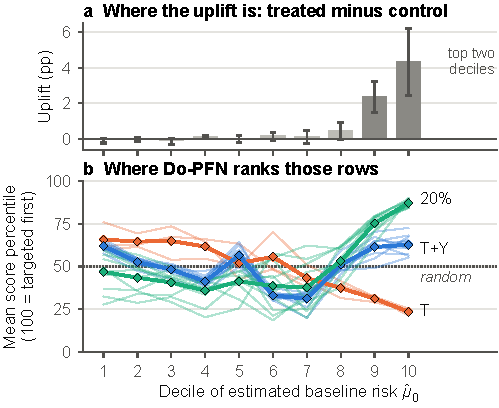
\includegraphics[width=\columnwidth]{figures/fig3_anatomy.pdf}
  \caption{Anatomy of the inversion on the 200k-row holdout subsample. (a)~Observed uplift by decile of estimated baseline risk \muz, with 95\% normal intervals. (b)~Mean percentile of Do-PFN's score within each decile; lines show the mean and bands the range across contexts (3 for T, 10 for \TY and 20\%). Under T, Do-PFN ranks the most responsive users near the bottom.}
  \label{fig:anatomy}
\end{figure}

\section{RQ4: Tuning the share, and its limits}

We selected the 20\% share on CV. On the holdout subsample it beats \TY in all 10 contexts tried: \Qhat is 0.074 against 0.049, a gain of $+0.025$\ci{0.015}{0.034}, with $+1.2$\pp\ci{0.3}{2.0} in uplift@10\% (Table~\ref{tab:holdout}). A two-level bootstrap that resamples contexts and row clusters together keeps the \Qhat gain positive\ci{0.005}{0.043} but leaves the uplift@10\% gain unresolved ($[-0.1,\,2.4]$\pp). Three of the contexts repeat the first check on a different GPU and agree with it within 0.001 in \Qhat. Four limits keep \TY as the default repair:

\emph{Data-rich learners stay ahead.} At 20\%, Do-PFN's \Qhat is 0.008 below that of a HistGB S-learner fitted on 2M development rows; the gap is resolved over contexts\ci{0.003}{0.013} but not once rows are resampled too ($[-0.006,\,0.022]$). Do-PFN's appeal lies in reading 1,024 rows, not in beating a learner that sees 2,000 times more.

\emph{Scores rank but do not estimate.} At 20\% the mean predicted effect is 6--7\pp, against an observed 1.0\pp.

\emph{The tuned share does not transfer.} On LZD, the CV optimum is 50\%, and 20\% is worse than \TY by 0.026. The signal on LZD is weak and noisy throughout.

\emph{Selection on CV is fragile.} In a separate check, 10 of 15 configurations chosen on CV scored lower on the holdout. The CV leader, the TabPFN T-learner with T contexts at $K{=}4{,}096$, fell from 0.077 to 0.006.

\section{Discussion and limitations}

Our results suggest three practical rules for in-context uplift models on rare binary outcomes.
(1)~Before trusting a causal PFN's ranking, check its sign on held-out randomized data and try an outcome-balanced context, which costs nothing at inference time.
(2)~Report the context sampler and evaluate several contexts per design: on the Criteo holdout, the context seed alone moves CausalPFN and the TabPFN T-learner by a standard deviation of 0.04--0.05 in \Qhat.
(3)~Use the scores to rank, not as effect estimates.

The evidence has clear bounds. One dataset carries a reliable signal, and we test one released checkpoint with contexts of at most 4,096 rows. The holdout was not untouched, and the data lack two features. The binary outcome lies outside Do-PFN's documented regime. Why the alignment with risk flips remains open. Per-arm predictions, other checkpoints and retrieved rather than sampled contexts~\cite{thomas2024retrieval} are the natural next steps.

\section*{Ethics statement}
We use public, anonymized data from randomized trials and collect no new data. Uplift models decide who receives ads or incentives. An inverted ranking wastes budget and gives incentives to the users least affected by them, so a model's ranking direction should be validated on randomized holdout data before deployment.

% Generative AI disclosure (ACM policy): describe here how AI tools were used in preparing the paper, if required.

\bibliographystyle{ACM-Reference-Format}
\bibliography{refs}

\end{document}
